\chapter{Proposed Methodology}
\label{ch:methodology}

This chapter presents the complete technical description of the proposed system in
three parts. Section~\ref{sec:prelims} reviews the building blocks required to
understand the construction. Section~\ref{sec:ibfv_arch} presents the IBFV
architecture---enrollment, verification, and the formal zero-penalty theorem.
Section~\ref{sec:dibfv_arch} describes the D-IBFV decentralized extension.

% ============================================================================
\section{Preliminaries}
\label{sec:prelims}
% ============================================================================

\subsection{Elliptic Curve Cryptography}
\label{sec:ecc_prelim}

An elliptic curve $E$ over a prime field $\mathrm{GF}(p)$ is defined by:
\begin{equation}
  y^2 \equiv x^3 + ax + b \pmod{p}
\end{equation}
The points on $E$, together with the point at infinity $\mathcal{O}$, form an
abelian group under the chord-and-tangent law. The security of elliptic curve
cryptography rests on the \textbf{Elliptic Curve Discrete Logarithm Problem}
(ECDLP): given a generator $G$ and a point $Q = s \cdot G$, finding the scalar
$s$ is computationally infeasible. For a 256-bit group, the best known attack
(Pollard's rho) requires approximately $2^{128}$ group operations.

This thesis uses \textbf{Brainpool~P256r1} \cite{rfc5639}, a 256-bit curve
standardized by the German Federal Office for Information Security (BSI) with
prime order $n$, cofactor $h = 1$, and no known special-purpose attack speedups.
A key property exploited in the vault construction is that mapping a minutia
$q_i$ to the curve point $P_i = q_i \cdot G$ is a one-way function: recovering
$q_i$ from $P_i.x$ (the $x$-coordinate stored in the vault) requires solving ECDLP.

\subsection{ECC-Based Fuzzy Vault}
\label{sec:ecc_vault_prelim}

The fuzzy vault \cite{juels2002fuzzy} binds a secret to a noisy, unordered
biometric set $\mathcal{Q}$ by evaluating a degree-$k$ polynomial $p(x)$ at
biometric-derived coordinates and hiding the resulting genuine points among
randomly generated chaff that do not lie on $p(x)$. Unlocking requires
identifying at least $k{+}1$ genuine points for Lagrange interpolation.

The ECC vault construction of Maurya et al.\ \cite{maurya2025enhancing} is
adopted as the baseline:

\subsubsection{Enrollment (Locking)}
\begin{enumerate}
  \item \textbf{Quantization}: Each minutia $m_i = (x_i, y_i, \theta_i)$ is
  quantized by factor $f$:
  \begin{equation}
    q_i = \left(\left\lfloor\frac{x_i}{f}\right\rfloor \bmod 64\right) \|
          \left(\left\lfloor\frac{y_i}{f}\right\rfloor \bmod 64\right) \|
          \left(\left\lfloor\frac{\theta_i}{f}\right\rfloor \bmod 64\right)
  \end{equation}
  producing an 18-bit integer. Duplicate values are removed to yield
  $\mathcal{Q} = \{q_1, \ldots, q_g\}$.

  \item \textbf{EC Mapping}: Each $q_i$ is mapped to a curve point
  $P_i = q_i \cdot G$, protected by ECDLP.

  \item \textbf{Polynomial Generation}: A random degree-$k$ polynomial
  $p(x) = \sum_{j=0}^{k} a_j x^j$ is generated over $\mathrm{GF}(p)$ with
  coefficients $a_j \in [10,63]$ (6~bits each). The secret key is
  $s = \left(\bigoplus_{j=0}^{k} \mathrm{bin}_6(a_j)\right) \bmod n$,
  and the public key is $S = s \cdot G$.

  \item \textbf{Genuine Points}: $\mathcal{G} = \{(P_i.x,\, p(P_i.x))\}_{i=1}^g$.

  \item \textbf{Chaff}: $5g$ points $(c_j.x, r_j)$ where $r_j \neq p(c_j.x)$.

  \item \textbf{Vault}: $\mathcal{V} = \mathrm{shuffle}(\mathcal{G} \cup \mathcal{C})$;
  stored as $(\mathcal{V}, S)$.
\end{enumerate}

\subsubsection{Verification (Unlocking)}
Query minutiae $\mathcal{M}'$ are quantized to $\mathcal{Q}'$; matching vault
x-coordinates $\mathcal{X}_m$ are found. If $|\mathcal{X}_m| \geq k{+}1$, each
$(k{+}1)$-subset is tested by Lagrange interpolation; the vault opens if the
reconstructed public key matches $S$.

\subsection{Iris Code Extraction}
\label{sec:iris_extract_prelim}

Iris images from CASIA-Iris-Interval ($320 \times 280$ pixels, near-infrared
illumination) are processed through a custom pipeline:

\begin{enumerate}
  \item \textbf{Segmentation}: The pupil boundary is detected via intensity
  thresholding; the outer iris boundary is located via a radial gradient search.
  A noise mask excludes the pupil interior, specular reflections, and eyelid
  occlusions (detected via column-wise variance on the normalized strip).

  \item \textbf{Normalization}: The annular iris region is unwrapped to a
  $64 \times 512$ rectangular strip using Daugman's rubber-sheet model
  \cite{daugman2004how}.

  \item \textbf{Encoding}: The strip is enhanced via CLAHE and encoded with 1-D
  Log-Gabor filters at two wavelengths (18 and 36 pixels, $\sigma/f = 0.30$),
  producing a phase-quantized binary iris code of
  $64 \times 512 \times 2 \times 2 = 131{,}072$ bits.
  Fragile bits (near phase boundaries, amplitude below $0.55\times$ the median)
  are masked \cite{hollingsworth2009fragile}; mean valid bit coverage is
  approximately 26\%.

  \item \textbf{Matching}: Iris codes are compared via fractional Hamming distance
  (FHD) over mutually valid bits, with circular shifts $(\pm 32)$ columns to
  compensate for rotational misalignment.
\end{enumerate}

\subsection{Iris Fuzzy Commitment with Bit Interleaving}
\label{sec:iris_commit_prelim}

A repetition-code fuzzy commitment extracts a stable binary key from an iris code.
Let $\mathbf{c} \in \{0,1\}^N$ be the $N$-bit iris code ($N = 131{,}072$) and
$B_s$ the block size. The number of blocks is $n_b = \lfloor N/B_s \rfloor$, each
contributing one key bit.

\subsubsection{Enrollment}
\begin{enumerate}
  \item Partition the iris code into $n_b$ blocks using \textbf{interleaved}
  assignment: bit $j$ belongs to block $(j \bmod n_b)$. This distributes
  spatially correlated noise across blocks rather than concentrating it in
  contiguous regions.
  \item Generate a random $n_b$-bit key $\mathbf{k}$.
  \item Construct repetition codeword $\mathbf{w}$: position $j$ is set to
  $k_{j \bmod n_b}$.
  \item Compute and store helper data $\mathbf{h} = \mathbf{c} \oplus \mathbf{w}$
  and key hash $H(\mathbf{k})$ (SHA-256).
\end{enumerate}

\subsubsection{Recovery}
For each rotation shift $\delta \in [-32, +32]$:
\begin{enumerate}
  \item Compute $\tilde{\mathbf{c}} = \mathrm{rotate}(\mathbf{c}', \delta)$ and
  $\tilde{\mathbf{w}} = \tilde{\mathbf{c}} \oplus \mathbf{h}$.
  \item For each block $i$, recover $\hat{k}_i$ by majority vote over the block's
  valid positions (masking fragile bits). With $B_s = 255$, the error capacity
  per block is $(B_s - 1)/2 = 127$ bit errors ($\sim$49.8\% error rate per block).
  Since genuine iris pairs exhibit FHD $\approx 0.20$ ($\sim$51 errors per
  255-bit block on average), majority vote succeeds for most blocks. For key
  recovery to succeed, all $n_b = 514$ blocks must decode correctly.
  \item If $H(\hat{\mathbf{k}}) = H(\mathbf{k})$, recovery succeeds.
\end{enumerate}
The resulting GAR is approximately 62\% and impostor FAR is approximately 0.10\%
at $B_s = 255$.

\subsection{Shamir's Secret Sharing}
\label{sec:shamir_prelim}

Shamir's $(t,n)$-threshold Secret Sharing \cite{shamir1979how} distributes a secret
$s \in \mathrm{GF}(q)$ among $n$ parties: evaluate a random degree-$(t{-}1)$
polynomial $f(x)$ with $f(0) = s$ at $n$ distinct points $\{(j, f(j))\}_{j=1}^n$.
Any $t$ shares suffice for exact Lagrange reconstruction of $s$; any $t{-}1$ or
fewer shares reveal zero information (information-theoretic security, regardless of
the adversary's computational power).

In D-IBFV, Shamir sharing is applied independently to each byte of the serialized
vault over $\mathrm{GF}(257)$---the smallest prime field that contains all 256 byte
values (0--255). Using uint16 encoding, each share is $2 \times$ the original
byte size.

\subsection{Blockchain and IPFS Infrastructure}
\label{sec:bc_ipfs_prelim}

\subsubsection{Hyperledger Fabric}
Hyperledger Fabric \cite{androulaki2018hyperledger} is a permissioned blockchain
with pluggable consensus (Raft, BFT) and chaincode (smart contract) execution.
Its execute-order-validate model is suitable for institutional deployments.
In D-IBFV, a Go chaincode manages CID storage, lookup, and revocation on a
Fabric channel, with Raft consensus and a 0.5-second block timeout.

\subsubsection{EVM-Compatible Platforms}
Ethereum \cite{buterin2014ethereum} and its local development proxy (Ganache)
provide permissionless smart-contract execution via Solidity. The same Solidity
contract deployed on Ganache is EVM-compatible with Polygon, Arbitrum, and other
Layer-2 chains. Ganache's instant block mining provides a controlled baseline for
latency measurements.

\subsubsection{IPFS}
IPFS \cite{benet2014ipfs} is a content-addressed storage network where each object
is identified by its SHA-256-based Content Identifier (CID). Storing a Shamir
share on IPFS provides: (a)~integrity---any tampering changes the CID; and
(b)~decentralization---the share can be retrieved from any node that pins it.
In D-IBFV, each of the $n$ Shamir shares is stored as a separate IPFS object;
the $n$ CIDs are anchored on the blockchain.

% ============================================================================
\section{IBFV Architecture}
\label{sec:ibfv_arch}
% ============================================================================

\subsection{Motivation: The AND-Fusion Penalty}
\label{sec:and_penalty}

Consider a conventional multimodal fuzzy vault where the iris serves as a
mandatory gate. Let $\mathrm{GAR}_\mathrm{FP}$ and $\mathrm{GAR}_\mathrm{Iris}$
denote the genuine acceptance rates of the fingerprint and iris subsystems.
Under AND-fusion:
\begin{equation}
  \mathrm{GAR}_\mathrm{AND} = \mathrm{GAR}_\mathrm{FP} \times
  \mathrm{GAR}_\mathrm{Iris} \leq \mathrm{GAR}_\mathrm{FP}
  \label{eq:and_penalty}
\end{equation}
Since $\mathrm{GAR}_\mathrm{Iris} < 1$ in practice (approximately 62\% in this
work), the AND-fusion combined system always performs worse than the unimodal
fingerprint for genuine users. Figure~\ref{fig:and_vs_ibfv} illustrates the
contrast between AND-fusion (gating) and IBFV (boosting).

\begin{figure}[h]
  \centering
  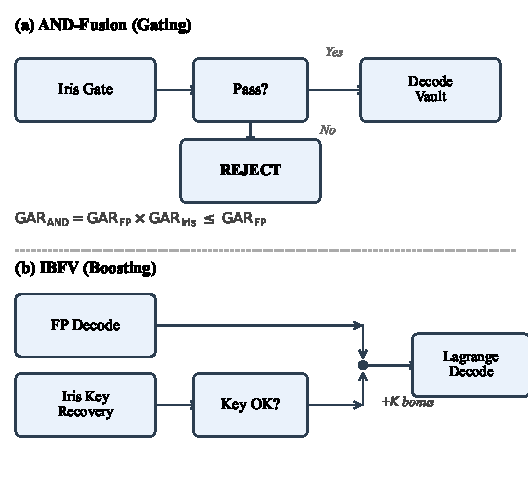
\includegraphics[width=0.9\linewidth]{figures/fig_and_vs_ibfv.pdf}
  \caption{AND-fusion vs.\ IBFV. (a) AND-fusion gates decoding: iris failure
  blocks the user. (b) IBFV boosts decoding: iris success adds $K$ bonus points;
  iris failure falls back to unimodal with zero penalty.}
  \label{fig:and_vs_ibfv}
\end{figure}

The same gating problem affects the three alternative tight-coupling architectures:
\begin{itemize}
  \item \textbf{Architecture B (Polynomial Blinding)}: The polynomial is
  XOR-masked with an iris-derived key; decryption requires iris key recovery.
  \item \textbf{Architecture C (Dense Chaff Seeding)}: The iris key seeds a
  PRNG for $20\times$ chaff inflation; without the iris key, the search space
  for polynomial reconstruction is $20\times$ larger.
  \item \textbf{Architecture D (AES-256-GCM Encryption)}: The vault is
  AES-256-GCM encrypted with the iris key; decryption is impossible without
  iris recovery.
\end{itemize}
All three require the iris for decoding, creating an AND-fusion constraint.

\subsection{IBFV Enrollment}
\label{sec:ibfv_enroll}

Given fingerprint minutiae $\mathcal{M}$ and iris code $(\mathbf{c}, \mathbf{mask})$,
enrollment proceeds as follows (see also Figure~\ref{fig:ibfv_enrollment}):

\begin{enumerate}
  \item Execute standard ECC vault enrollment (Section~\ref{sec:ecc_vault_prelim})
  to obtain genuine points $\mathcal{G}_\mathrm{FP}$, polynomial $p(x)$, and
  public key $S$.
  \item Perform iris fuzzy commitment enrollment (Section~\ref{sec:iris_commit_prelim})
  to obtain helper data $(\mathbf{h}, H(\mathbf{k}))$ and key hash $\kappa = H(\mathbf{k})$.
  \item \textbf{Derive virtual x-coordinates}: For $j = 0, \ldots, K{-}1$:
  \begin{equation}
    v_j = \mathrm{SHA}\text{-}256\!\left(\texttt{"ibfv\_vpt:"} \| j \| \texttt{":"} \| \kappa\right) \bmod p
    \label{eq:virtual_x}
  \end{equation}
  ensuring $v_j \notin \{P_i.x\}$ and all $v_j$ are distinct.
  \item \textbf{Compute bonus points}: $\mathcal{G}_\mathrm{Iris} =
  \{(v_j, p(v_j))\}_{j=0}^{K-1}$. These are genuine evaluation points of $p(x)$
  seeded by the iris key.
  \item \textbf{Generate chaff}: $5|\mathcal{G}_\mathrm{FP}|$ chaff points (chaff
  count based on fingerprint points only, not inflated by bonus points).
  \item \textbf{Construct vault}: $\mathcal{V} = \mathrm{shuffle}
  (\mathcal{G}_\mathrm{FP} \cup \mathcal{G}_\mathrm{Iris} \cup \mathcal{C})$.
\end{enumerate}

The stored vault is $(\mathcal{V}, S, \mathbf{h}, H(\mathbf{k}), B_s)$.

\begin{figure}[h]
  \centering
  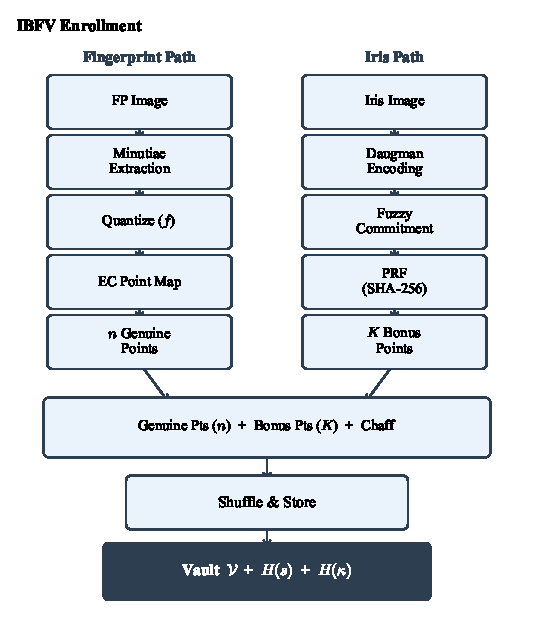
\includegraphics[width=0.9\linewidth]{figures/fig_ibfv_enrollment.pdf}
  \caption{IBFV enrollment pipeline. The fingerprint path maps minutiae to EC
  points on Brainpool~P256r1. The iris path extracts a key via fuzzy commitment,
  seeding a PRF to derive $K$ bonus points. All points are merged with chaff.}
  \label{fig:ibfv_enrollment}
\end{figure}

\subsection{IBFV Verification}
\label{sec:ibfv_verify}

Given query fingerprint $\mathcal{M}'$ and iris code $(\mathbf{c}', \mathbf{mask}')$:

\begin{enumerate}
  \item Quantize query minutiae; find FP-matching vault points:
  $\mathcal{X}_\mathrm{FP} = \{(x,y) \in \mathcal{V} : x \in \mathrm{EC}(\mathcal{Q}')\}$.
  \item Attempt iris key recovery (Section~\ref{sec:iris_commit_prelim}).
  \item \textbf{If iris succeeds} (key $\hat{\mathbf{k}}$ recovered):
    \begin{enumerate}
      \item Derive virtual x-coordinates $\{v_0, \ldots, v_{K-1}\}$ using
      Eq.~(\ref{eq:virtual_x}).
      \item Find bonus matches: $\mathcal{X}_\mathrm{Iris} = \{(x,y) \in \mathcal{V}
      : x \in \{v_j\}\}$.
      \item Total candidate set: $\mathcal{X} = \mathcal{X}_\mathrm{FP} \cup
      \mathcal{X}_\mathrm{Iris}$.
      \item \textbf{Smart decoding}: Fix all $K$ bonus points (guaranteed genuine)
      and enumerate only the remaining $k{+}1{-}K$ points from
      $\mathcal{X}_\mathrm{FP}$, reducing the search space by $\approx\!5.5\times$
      for typical parameters ($k=10$, $K=4$, $|\mathcal{X}_\mathrm{FP}|=12$).
    \end{enumerate}
  \item \textbf{If iris fails}: Set $\mathcal{X} = \mathcal{X}_\mathrm{FP}$ and
  proceed with standard Lagrange interpolation---identical to the unimodal vault.
\end{enumerate}

\begin{figure}[h]
  \centering
  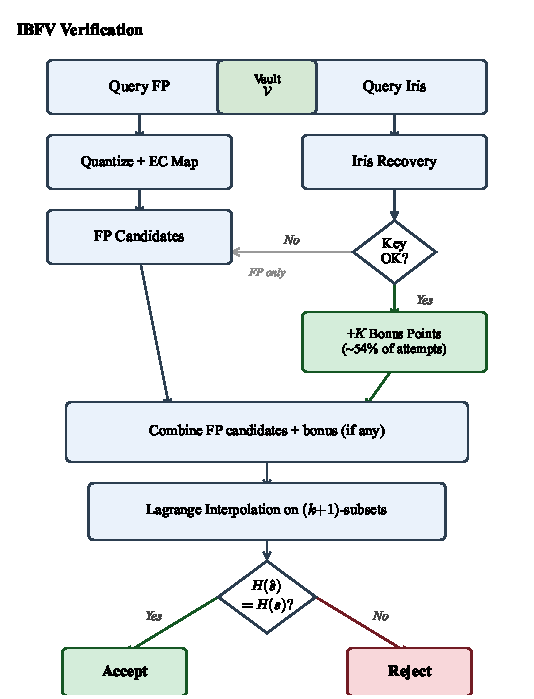
\includegraphics[width=0.9\linewidth]{figures/fig_ibfv_verification.pdf}
  \caption{IBFV verification pipeline. If iris recovery succeeds ($\sim$62\%),
  $K$ bonus points reduce the search space. If it fails (dashed path), the system
  falls back to unimodal decoding with zero penalty.}
  \label{fig:ibfv_verification}
\end{figure}

\subsection{Zero-Penalty Theorem}
\label{sec:zp_theorem}

\begin{mytherm}[Zero-Penalty Guarantee]
\label{thm:zp_theorem}
For any parameter configuration $(f, k)$ and any biometric sample pair
$(\mathcal{M}', \mathbf{c}')$, the IBFV verification outcome satisfies:
\begin{equation}
  \Pr[\mathrm{Accept}_\mathrm{IBFV}] \geq \Pr[\mathrm{Accept}_\mathrm{Uni}]
\end{equation}
where the probability is over the randomness in vault construction.
\end{mytherm}

\noindent\textit{Proof sketch.} If the iris succeeds, IBFV's candidate set
strictly contains the unimodal set, so any unimodal acceptance also triggers
IBFV acceptance. If the iris fails, decoding is identical to unimodal.
In neither branch does IBFV reject when the unimodal decoder would accept.
Complete proof in Appendix~A.

A corollary follows immediately: $\mathrm{FRR}_\mathrm{IBFV} \leq
\mathrm{FRR}_\mathrm{Uni}$ for all parameter settings. Since the iris impostor
FAR is near-zero ($\approx 0.10\%$ at $B_s = 255$), bonus points are almost never
injected for impostors, so $\mathrm{FAR}_\mathrm{IBFV} \approx \mathrm{FAR}_\mathrm{Uni}$,
and thus $\mathrm{EER}_\mathrm{IBFV} \leq \mathrm{EER}_\mathrm{Uni}$.

% ============================================================================
\section{D-IBFV: Decentralized Extension}
\label{sec:dibfv_arch}
% ============================================================================

\subsection{Motivation}
\label{sec:dibfv_motivation}

The IBFV vault is a high-value target: server compromise exposes every enrolled
user's vault to offline polynomial reconstruction attacks. D-IBFV eliminates
single-server trust by applying $(t,n)$-Shamir Secret Sharing to the entire vault,
storing shares on IPFS, and anchoring their integrity hashes on a blockchain ledger.
Figure~\ref{fig:dibfv_arch} shows the complete architecture.

\begin{figure}[h]
  \centering
  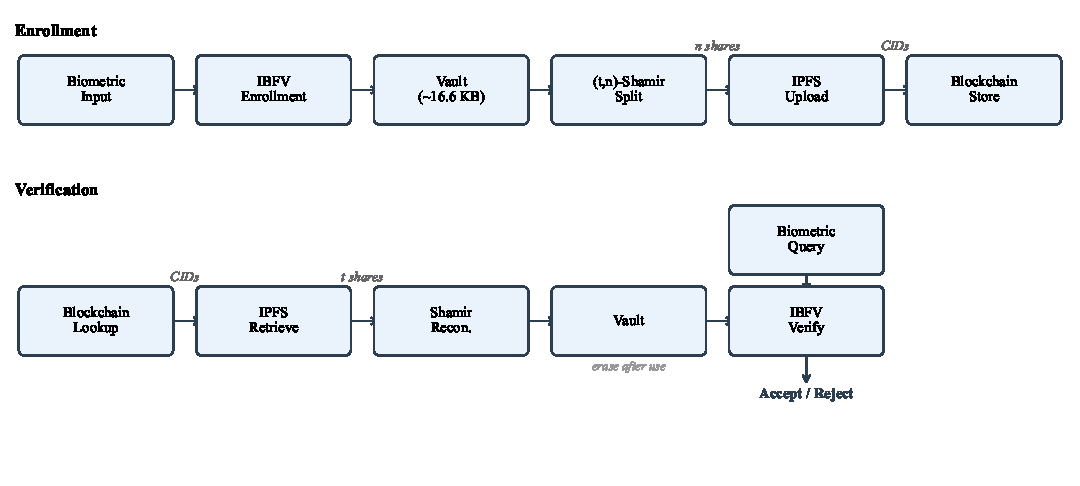
\includegraphics[width=0.9\linewidth]{figures/fig_dibfv_architecture.pdf}
  \caption{Complete D-IBFV architecture. Top: enrollment pipeline. Bottom:
  verification pipeline. The vault never exists as a complete unit on any single
  node except transiently on the trusted enrollment/verification client.}
  \label{fig:dibfv_arch}
\end{figure}

\subsection{Vault Serialization}
\label{sec:vault_serial}

The vault $(\mathcal{V}, S, \mathbf{h}, H(\mathbf{k}), B_s)$ is deterministically
serialized into a byte string $\mathbf{b} \in \{0, \ldots, 255\}^L$:
\begin{itemize}
  \item 8-byte header (parameters and format version)
  \item $|\mathcal{V}| \times 64$ bytes of vault point coordinates
  \item 64 bytes for the ECC public key $S$
  \item $\lceil N/8 \rceil$ bytes of iris helper data $\mathbf{h}$
  \item 32 bytes for the key hash $H(\mathbf{k})$
  \item 4 bytes of scheme parameters ($B_s$, $K$, $k$, $f$)
  \item 32-byte SHA-256 integrity trailer over all preceding bytes
\end{itemize}
For typical parameters ($g = 20$, $K = 4$, chaff $= 5g = 100$ points),
$L \approx 16.6$~KB.

\subsection{Shamir Vault Splitting}
\label{sec:shamir_splitting}

Each byte $b_i$ of $\mathbf{b}$ is independently shared over $\mathrm{GF}(257)$:
\begin{equation}
  f_i(x) = b_i + a_1^{(i)} x + \cdots + a_{t-1}^{(i)} x^{t-1} \pmod{257}
\end{equation}
with coefficients $a_j^{(i)} \stackrel{\$}{\leftarrow} \mathrm{GF}(257)$.
Share $j$ receives $(j, f_i(j))$ for each byte $i$.

Two theorems govern the security and correctness of this construction:

\begin{mytherm}[Share Confidentiality]
For any $t' < t$ compromised shares, the conditional distribution of vault
$\mathbf{b}$ is uniform over $\{0, \ldots, 255\}^L$. Fewer than $t$ shares
reveal zero information about the vault content.
\end{mytherm}

\begin{mytherm}[Exact Reconstruction]
\label{thm:exact_recon}
Given any $t$ shares with distinct indices, Lagrange interpolation over
$\mathrm{GF}(257)$ recovers $\hat{b}_i = b_i$ for all $i$, yielding
$\hat{\mathbf{b}} = \mathbf{b}$ with zero bit errors.
\end{mytherm}

Complete proofs are given in Appendix~A.

\subsection{Distributed Enrollment Protocol}
\label{sec:dist_enroll}

The enrollment protocol extends IBFV enrollment with three steps:

\begin{enumerate}
  \item Run IBFV enrollment to obtain the vault $(\mathcal{V}, S, \mathbf{h},
  \kappa, B_s)$.
  \item Serialize the vault to byte string $\mathbf{b}$.
  \item Apply $(t,n)$-Shamir splitting to obtain $n$ shares
  $\{\mathbf{s}_1, \ldots, \mathbf{s}_n\}$.
  \item Upload each share $\mathbf{s}_j$ to IPFS; record its CID $\mathrm{cid}_j$.
  \item Store $(\mathrm{uid}, \{\mathrm{cid}_1, \ldots, \mathrm{cid}_n\}, t, n)$
  on the blockchain.
  \item Securely erase $\mathbf{b}$ and all shares from local memory.
\end{enumerate}

The complete vault never exists on any server; only individual shares (which are
information-theoretically useless without $t{-}1$ others) are persisted.

\subsection{Distributed Verification Protocol}
\label{sec:dist_verify}

\begin{enumerate}
  \item Retrieve the CID list and threshold $t$ from the blockchain for the
  claimed user ID.
  \item Download any $t$ available shares from IPFS; verify each share against
  its CID (IPFS content addressing provides automatic integrity verification).
  \item Reconstruct $\hat{\mathbf{b}}$ via Lagrange interpolation over
  $\mathrm{GF}(257)$.
  \item Verify the SHA-256 integrity trailer embedded in $\hat{\mathbf{b}}$.
  \item Deserialize the vault from $\hat{\mathbf{b}}$.
  \item Run IBFV verification against the reconstructed vault.
  \item Securely erase $\hat{\mathbf{b}}$ and all shares from local memory.
\end{enumerate}

The reconstructed vault exists only transiently in memory on the verification
client and is erased immediately after the biometric decision.

\subsection{Revocation and Re-Enrollment}
\label{sec:revocation_design}

To revoke a compromised vault:
\begin{enumerate}
  \item Submit a revocation transaction to the blockchain, marking the current
  CID set as revoked. The blockchain's append-only nature provides a permanent,
  tamper-evident audit trail.
  \item Re-enroll with fresh parameters: a new polynomial, a new iris commitment
  key, and new Shamir randomness. By Theorem~2, new shares are information-
  theoretically independent of revoked shares.
  \item Upload new shares to IPFS; record new CIDs on the blockchain.
\end{enumerate}

\subsection{Extended Threat Model for D-IBFV}
\label{sec:extended_threats}

D-IBFV adds three attack points beyond the standard eight-point model:

\begin{itemize}
  \item \textbf{Node compromise}: An adversary compromises up to $t{-}1$ IPFS
  storage nodes. Countermeasure: Theorem~2 guarantees zero information leakage
  from $t{-}1$ or fewer shares.

  \item \textbf{Blockchain tampering}: An adversary attempts to modify CID records.
  Countermeasure: Blockchain consensus (Raft/BFT) makes retroactive modification
  computationally/information-theoretically infeasible. IPFS CIDs independently
  verify share integrity.

  \item \textbf{IPFS share substitution}: An adversary replaces a share blob.
  Countermeasure: IPFS CIDs are cryptographic content hashes; substitution
  changes the CID. The blockchain-anchored CID and the vault's SHA-256 integrity
  trailer jointly detect any corruption.
\end{itemize}

